\documentclass[oupdraft]{bio}
\usepackage[colorlinks=true, urlcolor=citecolor, linkcolor=citecolor, citecolor=citecolor]{hyperref}

% Add history information for the article if required
\history{Received August 1, 2010;
revised October 1, 2010;
accepted for publication November 1, 2010}

\begin{document}

% Title of paper
\title{Exploration of empirical Bayes hierarchical modeling for the
analysis of genome-wide association study data}

% List of authors, with corresponding author marked by asterisk
\author{ELIZABETH A. HERON$^\ast$, COLM O'DUSHLAINE, RICARDO SEGURADO,\\
LOUISE GALLAGHER, MICHAEL GILL\\[4pt]
% Author addresses
\textit{Neuropsychiatric Genetics Research Group and Department of Psychiatry,
Trinity College Dublin,
Trinity Centre for Health Sciences,
James's Street, Dublin 8,
Ireland}
\\[2pt]
% E-mail address for correspondence
{eaheron@tcd.ie}}

% Running headers of paper:
\markboth%
% First field is the short list of authors
{E. A. Heron and others}
% Second field is the short title of the paper
{Empirical Bayes hierarchical modeling for GWAS}

\maketitle

% Add a footnote for the corresponding author if one has been
% identified in the author list
\footnotetext{To whom correspondence should be addressed.}

\begin{abstract}
{In the analysis of genome-wide association (GWA) data, the aim is
to detect statistical associations between single nucleotide
polymorphisms (SNPs) and the disease or trait of interest. These
SNPs, or the particular regions of the genome they implicate, are
then considered for further study. We demonstrate through a
comprehensive simulation study that the inclusion of additional,
biologically relevant information through a 2-level
empirical Bayes hierarchical model framework offers a more robust
method of detecting associated SNPs. The empirical Bayes approach
is an objective means of analyzing the data without the need for
the setting of subjective parameter estimates. This framework
gives more stable estimates of effects through a reduction of the
variability in the usual effect estimates. We also demonstrate the
consequences of including additional information that is not
informative and examine power and false-positive rates. We apply
the methodology to a number of genome-wide association (GWA)
data sets with the inclusion of additional biological information.
Our results agree with previous findings and in the case of one
data set (Crohn's disease) suggest an additional region of interest.}
{Coronary artery disease; Crohn's disease; Multilevel model;
Rheumatoid arthritis; Semi-Bayes; Type 2 diabetes.}
\end{abstract}


\section{Introduction}
\label{sec1}

Genome-wide association studies (GWASs) aiming to detect
associations between observable traits and genetic variation
across the genome are now commonplace thanks to the advent of
several economically feasible high-throughput genotyping
technologies. This genetic variation is typically in the form of
single nucleotide polymorphisms (SNPs). Data consist of genotypes
at each of the SNPs, for members of groups of cases and controls
or family members (parents and affected offspring). The choice
of case-control or family data may depend on the age-of-onset
of the disease/trait being studied. There are many approaches to
analyzing these data, including, for example, single SNP
analyses and pathway approaches;
\citet{allison2006}
provide a review of current statistical analysis methodologies.
A typical study design consists of 2 stages: first, an association
analysis is carried out on each SNP, with the observed trait/phenotype
status. Then the SNPs deemed most highly associated with the trait,
and often additional surrounding SNPs are analyzed in independent
samples in order to determine whether or not the signals are
replicated.

The SNP data are analyzed in the case--control setting with one of a
range of statistical tests, for example, Cochran--Armitage trend
test, Cochran--Mantel--Haenszel test, logistic regression, and
Bayes factors. Each of these tests assume certain genetic models
and can account for the presence of population stratification and
any additional information that may be available for the individuals
in the study. The results from these analyses are usually in the
form of a ranked list of \textit{P}-values from which a subset of
the top ranked SNPs is then taken forward for further study in an
independent sample.

For each individual, as well as their genotype at each SNP,
additional information is often recorded, for example, age, sex,
and medical history. Also, as GWASs are often carried out
in large consortia, with sample collections taking place at
various sites, the site, and ethnicity information (sometimes
self-reported or inferred) are also available. These are just some
examples of extra data that may have been recorded, and we will
henceforth refer to this type of additional information as
additional phenotypic information (additional to the disease or
trait status). This additional phenotypic information should,
where possible, be incorporated into the testing for SNP
association.

In these analyses, all SNPs are treated in the same manner; in
particular, they are all modeled as being equally likely to have
the same impact on the phenotype. The exception being the Bayes
factor approach which, among other advantages, allows for the
inclusion of prior association information for each SNP. Although
these analyses do sometimes incorporate additional phenotypic
information such as that described above, rarely is other
additional biological information included.

This biological information may be in the form of functional
information, for example, biologically relevant location
information for the SNPs, prior linkage findings, or prior
association findings. This type of additional information
that relates to the SNPs as opposed to the individuals in the
study will be referred to as additional biological information.
Approaches have been proposed to include this additional
biological information in the form of multilevel or hierarchical
models
(\citealp{Duditetal02,rma2003,LW2004,rieger2004}).

Hierarchical or multilevel modeling, as the names suggest,
consist of 2 or more levels that are organized in a
hierarchical framework. The levels specify relationships between
the variables and parameters that are of interest; these
relationships may be in the form of regression equations, for
example. The estimation of parameters in these models can be
carried out in a fully Bayesian manner, where the distinction
between data and prior information is strictly adhered to, with
the prior distribution not depending on the data. A semi-Bayes
approach can also be used in which prior information is
subjectively fixed by the practitioner or an empirical Bayes
approach in which the data themselves are used to specify priors.
This latter approach can be thought of as lying somewhere between
the fully Bayes and semi-Bayes approaches. Many authors in
various fields have advocated the use of hierarchical models,
and we suggest
\citet{tomlins2005},
\citet{TTC01}
and
\citet{Barlow_Bartholomew:1972}
both for introductions to hierarchical models and for more
formal and detailed accounts.

Hierarchical modeling approaches offer many advantages over
conventional methods. The ability to, easily and in a coherent
framework, include relevant additional information---information
that will help to inform on the disease/trait of interest---is one
of the main advantages of this methodology. Hierarchical models
offer better and more stable estimates of parameters than
conventional methods. In general, estimates that are extreme
and/or unstable become more reasonable in the hierarchical model
setting and those parameter estimates that are more moderate
remain so in the hierarchical approach
(\citealp{Gichangi_Vach:2006}).

As previously mentioned, the \textit{P}-value is the predominant
measure used in ranking GWASs. Other authors have advocated
using effect sizes rather than \textit{P}-values in various
settings, including in the detection of influential genetic
markers
(\citealp{rieger2004,tomlins2005,TTC01}).
In the present context, the effect size can
be thought of as indicating the ``quantitative importance''
(\citealp{Gichangi_Vach:2006})
of the association. On the other hand, the \textit{P}-value
does contain information on the magnitude of the effect
size but this is confounded by the fact that it also
contains information on the precision with which the effect
size is measured. For example, 2 markers having the same
\textit{P}-values may have very different effect sizes as a
result of having very different minor allele frequencies (MAFs).
Thus, it is clear that the use of \textit{P}-values for ranking
associations may not always be ideal. As well as being useful for
the prediction of risk, the empirical Bayes hierarchical effect
estimates can potentially be used in the ranking of associations
and in the goal of false-positive reduction.

In the present context, the hierarchical modeling approach
permits the relaxation of the assumption that all SNPs act
similarly and allows for the SNP effects to vary, depending on
the additional genetic information. Incorporating this additional
information should help to control for false-positive associations
that may be observed using conventional tests. Here, we present
a 2-level hierarchical model and, depending on how the model
is viewed, the interpretation of the role of the additional
biological information may change. For example, in the
frequentist setting, the multilevel model can be viewed as a
mixed model with both fixed and random effects. If on the other
hand, the model is viewed from a Bayesian perspective, the
additional genetic information may be entering the model in
the form of a prior distribution (see Section \ref{sec1} of
the supplementary material [SM] available at
\textit{Biostatistics} online).

Earlier hierarchical modeling approaches allowing for the
incorporation of additional biological information for smaller
scale association studies include
\citet{Barlow_Bartholomew:1972},
who used a logistic regression model for the first level,
in an SNP association study for candidate genes in bladder
cancer. As well as including biological factors in the second
level of the model, the authors also included environmental
factors and considered interaction effects in the first level.

\citet{Wahba:1990}
provide a hierarchical regression modeling approach, the first
level of which is based on the positive root of a 1-degree of
freedom (df) $\chi^2$ statistic, $x_m$, which has a noncentral
$\chi$ distribution with 1 df and noncentrality parameter
$\lambda_m$. The $\lambda_m$, which are of main interest,
indicate the strength of association and in turn are modeled
using a mixture model, allowing the incorporation of any prior
knowledge of association. The prior depends on additional
covariate information such as, for example, whether the marker
is located in an exon, or a splice junction site, its predicted
effect on protein conformation, or prior linkage, or association
evidence. The authors compare various empirical and fully
Bayesian schemes for this modeling framework using simulated
data, where performance is assessed in terms of power.

\citet{Brown:1989}
also propose a 2-level hierarchical modeling approach and explore
both empirical Bayes and semi-Bayes approaches. For their empirical
Bayes approach, they develop a structured weighting function
that reflects the residual variation in the first-level estimates
that remains after the second-level covariates have been taken
into account. This weighting function is designed to give more
support to particular markers based on one or more different
types of additional biological information. For example, those
markers with higher previous linkage or association scores may
be weighted more heavily. They apply their methods to both GWA
SNP data and gene expression data.

\citet{SAS_Institute:1999}
presents both empirical Bayes and semi-Bayes adjustments that
shrink the conventional effect estimates toward an overall
average effect. For the empirical Bayes method, rather than
using additional covariate information, the author sets the prior
mean effect for all SNPs to be zero. The author applies the
method to a GWAS on Type 2 diabetes (T2D) with the first-level
estimates arising from the Cochran--Armitage test for trend.
The author also explores a semi-Bayes approach.

Most of the analyses cited above consider the application of the
empirical Bayes hierarchical model (EB-HM) to experimental data
sets only and, even where they do include the use of additional
covariate information, do not present any exploration of the
sensitivity of the approach to this information. The exception is
\citet{Fimmers_Seuchter:1989}
who in contrast do not present any application to experimental
data but restrict their attention to simulation studies. In
this paper, we aim to bridge the gap between simulated and
experimental GWA data by developing a straightforward model
that facilitates clearer comparison of the behavior of the
methodology between both data types. In particular, we examine
the impact of the inclusion of both informative and
noninformative additional information. We are presenting a
widely applicable methodology to incorporate additional biological
information that allows the nonsubjective determination of the
influence of this additional information. The methodology provides
effect estimates that can be used for ranking purposes to
prioritize markers for further study.

We present a 2-level EB-HM for the analysis of individual
marker GWA data, focusing on the case--control study design.
This modeling framework consists of a first-level logistic
regression model for each individual SNP with a second-level
regression, incorporating additional biologically relevant
information. An empirical Bayes approach, using techniques
proposed by
\citet{Barlow:1972},
to iteratively estimate prior parameters in the model using
the available data, is proposed. A key advantage of this
empirical Bayes approach is that it does not rely on the
subjective input of the practitioner in setting prior
information but instead uses the available data to obtain
parameter estimates. Previous examinations of the empirical
Bayes approach have highlighted the conservative nature of
the methodology, in particular when compared to the subjective
semi-Bayes approaches
(\citealp{Castelloe_Zimmerman:2002,Schwender:2007}).
We acknowledge that our objective approach presented here
is conservative and, in our implementation, results in
effect sizes (odds ratios) that may be underestimated. Our
simulation studies present evidence of this; however, this
conservatism does not compromise the ranking and identification
of associated markers---as evidenced in both our simulation and
experimental data applications.

We explore a comprehensive simulation study that shows the
effectiveness of our approach when truly relevant additional
biological information is included. We also demonstrate, through
simulations, the effect of applying this methodology when noisy,
incomplete information is included. Although we do not incorporate
linkage disequilibrium (LD) in our simulation studies, we do not
feel this is a major drawback. In identifying variants that are
associated with the phenotype of interest, the usual single-level
approach can result in a set of markers being identified that are
correlated with each other to varying degrees. Each of these
variants is not usually treated as a separate association signal
but rather the region is identified. If LD is of concern, the
approach of LD pruning could first be employed---resulting in a
set of independent, uncorrelated markers. Also, markers that are
in LD with those in functional regions can be identified and such
information incorporated in the additional covariate information,
as we demonstrate in our experimental data applications. We also
assess our proposed model extensively in terms of power and
false-positive rates under various scenarios. We conclude by
applying the methodology to 4 of the Wellcome Trust Case
Control Consortium data sets: T2D, coronary artery disease
(CAD), Crohn's disease (CD), and rheumatoid arthritis (RA)
(\citealp{allison2006}).


\section{Methods}
\label{sec2}

In our development of the methodology for the hierarchical model,
we will concentrate on the case--control study design. Here, we
present a 2-level EB-HM. The first level comprises a logistic
regression model, and the second level comprises a Gaussian
regression incorporating additional biologically relevant
information.


\subsection{First level---logistic regression}

The first level, in the 2-level hierarchical model for
case--control type data, consists of the analysis of the
individual SNPs; independently testing for associations between
the individual SNP markers and case--control status. Given $N$
individuals, a proportion of which will be cases and the remaining
individuals controls, proportions that need not necessarily be
equal, for each of the $M$ SNPs we propose using a logistic
regression model to test for association. The logistic regression
model is chosen as it is a flexible model choice, allowing for the
incorporation of various genetic models (e.g., additive,
recessive, and dominant) which may be thought to underlie the
disease or trait under consideration. The logistic regression
approach also allows for the inclusion of additional phenotypic
information through the inclusion of additional covariates. For
the phenotype data (case--control status), for $i = 1, \ldots, N$
individuals, let $y_i = 1$, if individual $i$ is a case,
and let $y_i = 0$, if individual $i$ is a control. For the
genotype data, for $m = 1, \ldots, M$, we let $X_{mi}$
denote the genotype for individual $i$ at marker $m$. The
genetic model may be incorporated here through the
choice of coding for the number of minor alleles (from here on
referred to as the allele) at the particular marker locus. For
example, for an additive model, $X_{mi}$, takes the values 0, 1,
or 2, indicating 0, 1, or 2 copies of the allele. For a
dominant model, $X_{mi}$ can take the values 0 or 1, 0
indicating 0 copies of the allele and 1 indicating one or
2 copies of the allele. Similarly, other genetic models
may be incorporated.

The logistic regression model is given by the following
equation:
\begin{equation}
\log \left( \frac{p_{mi}}{1 - p_{mi}} \right)
= \hbox{logit} (p_{mi})
= \alpha_m + \beta_m X_{mi},
\label{logistic regression}
\end{equation}
where $p_{mi}$ is the probability of individual $i$ being a
case given that they have genotype $X_{mi}$ at marker $m$.
$\alpha_m$, the baseline risk of disease, is the log odds for
an individual having the disease given that they have the
homozygous genotype for the major allele (i.e., they have 0
copies of the minor allele). The $\beta_m$ are an estimate
of the increase in odds of being a case for each additional
allele (assuming additive model) on the log-odds scale and
are thus an estimate of the effect size. Where available,
additional phenotypic information, such as that previously
mentioned, may be incorporated through the inclusion of
additional covariates and their corresponding coefficients
in (\ref{logistic regression}), but for simplicity, we
will not include these here. The statistical significance
of the association can be tested using the Wald statistic,
given by
$\left( \hat{\beta}_m / \hbox{SE} (\hat{\beta}_m) \right)^2
\sim \chi^2$,
where $\hat{\beta}_m$ is the maximum likelihood estimator
(MLE) of $\beta_m$ and
$\hbox{SE} \left( \hat{\beta}_m \right)$
is its associated standard error. In the usual approach
to analyzing GWAS data, the resulting \textit{P}-values
would be ranked in ascending order, and a \textit{P}-value
threshold (such as genome-wide significance;
\citealp{Duditetal02})
used in order to determine which SNPs to investigate
further. A logistic regression model has been used in
\citet{rma2003},
\citet{LW2004},
and
\citet{rieger2004},
for example, to detect SNP associations in GWASs for
various diseases. Our aim is to include additional
biologically relevant information in our analysis through the
incorporation of a second-level regression equation in our model.


\subsection{Second level---regression}

The second level of the model aims to improve the estimates
of the $\beta_m$ through the inclusion of additional biological
information. This is facilitated through the inclusion of
a second regression equation given by
\begin{equation}
\beta = Z \gamma + \tau^2 T,
\quad
\beta = \left( \beta_1, \ldots, \beta_M \right),
\quad
\beta_m \sim \hbox{Normal} \left( Z_m \gamma, \tau^2 t_{mm} \right),
\label{second level}
\end{equation}
where $Z$ is an $M \times K$ matrix containing $K$ columns of
additional biological information. Thus, for each $\beta_m$
(and thus each marker $m$), there is information on each of
the additional biologically relevant covariates. There is no
restriction on the values the entries in the matrix $Z$ can
take. For example, negative entries could be used to indicate
that a particular covariate was expected to have a negative
or opposite effect (protective) in contributing to
susceptibility to disease. For the type of information
included in $Z$, it will often be the case that many of the
entries will be binary, indicating membership of a particular
functional class, for example, SNPs in introns.

The vector $\gamma$ is a $K \times 1$ vector of second-level
regression coefficients. $\tau^2 T$ is a variance--covariance
matrix representing the residual variation in the $\beta_m$'s
that remains after the second-level covariates in the $Z$ matrix
have been taken into consideration. Thus, $\tau^2 T$ reflects
any unmodeled and unaccounted-for variability which could be due
to, for example, interaction effects between the second-level
covariates or covariates not included. Correlation structure
between the SNPs would be modeled in the off-diagonal entries of
the $T$ matrix. If no correlation structure is to be modeled,
which can reduce the computational burden, then $T$ can be
defined as the identity matrix.
\citet{tomlins2005}
follow a similar rationale in defining $T$.

In Section \ref{sec1} of the SM available at
\textit{Biostatistics} online, we explore the mixed model
and Bayesian interpretations of combining (\ref{logistic regression})
and (\ref{second level}) which can help clarify the roles played by
the various components of the model.


\subsection{Combining first- and second-level effect estimates}

We combine the first-level estimates and the second-level means
for the $\beta_m$ using the hierarchical estimator:
\begin{equation}
\hat{\beta}_{m; \mathrm{EB}} =
B_m Z_m \gamma + \left( 1 - B_m \right) \hat{\beta}_m.
\label{shrinkage}
\end{equation}
Equation (\ref{shrinkage}) is sometimes referred to as a
shrinkage estimator
(\citealp{TTC01})
because the first level usual
estimators, $\beta_m$, are shrunk toward, or averaged with,
the second-level means $Z_m \gamma$. The shrinkage factor
$B_m$ indicates how much the second-level mean $Z_m \gamma$
contributes to the estimate $\beta_m$.
\citet{Gichangi_Vach:2006},
in his analysis, sets $Z_m \gamma$ to be zero for all SNPs,
as it is felt that this could be a reasonable choice in GWAS
applications. If the first-level estimators are highly
variable, with respect to the total variability, they will
be shrunk toward the more stable estimate, $Z_m \gamma$,
thus reducing the variability. On the other hand, if the
logistic regression estimates have small variability, then
these estimates will not be shrunk as much toward the
second-level means. The important question is how to
determine the shrinkage factors $\{ B_m \}$. There are
various methods of choosing/estimating these, for example,
empirical Bayes, semi-Bayes, and fully Bayesian approaches.
Here, we will only concentrate on using an empirical Bayes
estimator. Just as the means for the second-level model are
estimated from the data, we will also estimate the prior means,
and consequently, the shrinkage factors, using the data.
This is in contrast to the semi-Bayes approach that would
rely on the subjective judgement of the data analyst in
setting the prior means.

We will use the empirical Bayes iterative approach described
in
\citet{Barlow_Bartholomew:1972}
to estimate the shrinkage factors. Further details are
given in Section \ref{sec2} of the SM available at
\textit{Biostatistics} online.


\subsection{Simulation strategy}

To evaluate and explore the performance of the approach
proposed here, we simulated case--control genotype data for
a number of markers. The multilevel format of the model allows
for a clear simulation framework, the natural starting point
for the simulation being the second-level regression equation.
Full details of the simulation strategy are given in
Section \ref{sec3} of the SM available at
\textit{Biostatistics} online.


\section{Results}
\label{sec3}

\subsection{Simulation study application}

To examine the efficiency of the proposed method for the better
identification of the associated markers, we simulated
case--control genotype data for 200 markers for each of 500
cases and 500 controls. We randomly simulated the MAFs on the
interval $(0.01, 0.5)$ and chose a dominant genetic disease
model with a disease prevalence of 0.05. Of the 200 markers,
3 markers were randomly chosen to have higher odds ratios
than all other markers (markers 44, 123, and 184). The matrix
$Z$ contained 5 columns of additional covariate information,
simulated from a Binomial distribution. The first column of
the $Z$ matrix was chosen as the most informative, and for
the randomly chosen markers, the corresponding entries in
this column of $Z$ were increased. The aim was to detect these
markers as associated markers, while also minimizing the
number of false positives. The results of this simulation
study can be seen in Figure \ref{Fig1}. The residual variation
that remains in the first-level coefficients, after the
second-level additional covariate information is included, is
modeled by $\tau^2$ and was set at 0.01 in the simulation
study. This is well estimated with the empirical Bayes approach
as $\hat{\tau}_2 = 0.00723$. As can be seen in Figure \ref{Fig1},
the EB-HM performs well in comparison to the MLEs of the
logistic regression model, both in the detection of the
markers with higher odds ratios and in the decrease of
false-positive findings through the reduction of the
standard errors.

We also compared the performance of the modeling framework
with respect to estimating the true odds ratios over a number
of random simulations. As noted by
\citet{Wahba:1990},
the effect estimates can be used for risk prediction and they
give an indication of the quantitative importance of putative
associations. To do this, we use the mean square error
$\hbox{MSE} = M^{-1}
\sum_m \left( \hbox{est(OR)} - \hbox{true(OR)}\right)^2$,
where the est(OR) is either the odds ratio as estimated by
the MLE from the logistic regression or the empirical Bayes
estimate of the odds ratio, and the true(OR) is the
simulated odds ratio. The MSE captures the degree to which the
estimator differs from the true odds ratio, which can either be
due to the stochastic nature of the process or the poor
performance of the estimator. We examine the MSE across 100 random
simulations for both the MLE and for the empirical Bayes
hierarchical modeling estimators and compare them in
Figure \ref{Fig1}(a) of the SM available at \textit{Biostatistics}
online. We also plot the proportion of MAFs that are $< 5\%$
in each simulation. This is done to explore the possibility
that simulations with many markers with low MAFs, which could
lead to decreased power to detect associations, may be
influential in the behavior of the estimators. There does
not appear to be any evidence for this.

The simulation studies so far have used the same $Z$ matrix,
containing the same additional covariate information, in
both the data simulation and the analysis phases. For
experimental data, it will almost always be the case that
such exact information will not be available. To examine
the situation where additional noisy and incomplete
information is provided in the analysis phase, we explored
the scenario where a different $Z$ matrix, $\hat{Z}$,
is used in the analysis stage to that used in the simulation
phase. In the simulation phase, $Z$ is used, but in the
analysis phase, we use $\hat{Z} = Z_{k - 1} + e$, where
$e \sim \hbox{Normal} (0, 1)$ and $Z_{k - 1}$ is the $Z$
matrix with one column of extra covariate information
omitted. All other parameters are similar to those in the
simulation studies described above. The results of this
simulation study can be seen in Figure \ref{Fig2}.
$\tau^2$ is set again at 0.01, and $\hat{\tau}^2$ is
estimated as 0.00584. The EB-HM still performs better
than the single-level MLE estimates from the logistic
regression. The aim would be that the empirical Bayes
model should not perform less well than the single-level
model, that is, that the additional noisy and incomplete
information should not lead to dramatically different
conclusions regarding which markers are believed to be
associated. For this simulation scenario, we also
simulated 100 random simulations and compared the
MSE for both the empirical Bayes estimators and the
MLEs. As can be seen in Figure \ref{Fig1}(b) of the
SM available at \textit{Biostatistics} online, the
empirical Bayes model still outperforms the single-level
logistic regression model when considering the estimation
of the odds ratios.

Finally, we show that the model does offer substantial
improvements over the usual single-level model by examining
the sensitivity and specificity of the model for simulated
data. We use receiver operating characteristic (ROC)
curves to assess these. In order to access the sensitivity
(power) and specificity (1 false-positive rate), we
generated 1000 random simulations, each having 2 random
markers (out of 200) with higher odds ratios and used the
same $Z$ covariate matrix in the analysis and generation
phases. We also carried out this same scenario for 15
random markers with higher odds ratios. As can be seen
from the ROC curves in Figure \ref{Fig3}(a) and (b),
EB-HM performs substantially better than the MLE when
relevant informative information is provided
(Figure \ref{Fig3}(a) area under curve [AUC] MLE: 0.896,
EB-HM: 0.998; Figure \ref{Fig3}(b) AUC MLE: 0.896,
EB-HM: 0.999). To assess the performance when
noninformative information is provided in the $Z$
covariate matrix, as may be the case in experimental
analyses, we also carried out the same simulation strategy
as just described but used positive random noise
($\hbox{abs} [ \hbox{Normal} (0, 1) ]$) for a reduced
number of covariates (5 columns in $Z$ in data generation
phase, and 4 columns in analysis phase). Examining
Figure \ref{Fig3}(c) and (d), it is clear that the model
is robust in the face of wrong, uninformative information
and performs just as well as the MLE method,
(Figure \ref{Fig3}(c) AUC MLE: 0.896, EB-HM: 0.889;
Figure \ref{Fig3}(d) AUC MLE: 0.897, EB-HM: 0.903).


\subsection{Application to WTCCC 2007 data sets}

We present applications of our methodology to CAD, CD,
RA, and T2D data sets from the
\cite{SAS_Institute:1999}.
Several of the genetic associations presented in
\citet{Brown:1989}
have been replicated. All data sets were quality controlled
to include SNPs with $\hbox{MAF} > 0.01$ and a
Hardy--Weinberg equilibrium threshold of $P < 10^{-4}$ in
both cases and controls. This resulted in 2938 controls
and CAD: 1926, CD: 1748, RA: 1860, and T2D: 1924 cases.
We examined autosomal SNPs (CAD: 380442, CD: 380664,
RA: 380481, and T2D: 380463) that had additional covariate
information available.

The covariate information that constitutes the $Z$ matrix
for each of these data sets consisted of 20 categories
of additional functional information for each SNP.
Specifically: 11 binary categories (Downstream, Essential
Splice Site, Intergenic, Intronic, Non-Synonomous Coding,
Regulatory Region, Splice Site, Stop, Synonomous Coding,
Upstream, and Untranslated Region (UTR)) and 9 linkage
disequilibrium sum (LDSUM) categories (LDSUM Downstream,
LDSUM Frameshift Coding, LDSUM Intergenic, LDSUM Intronic,
LDSUM Non-Synonomous Coding, LDSUMStop, LDSUM Synonomous
Coding, LDSUM Upstream, and LDSUM UTR). The scoring used
for the binary covariate categories is as follows. For
example, if an SNP scores a 1 for the intronic region,
this indicates that the SNP is contained in an intron,
similarly for the other binary categories. For a particular
marker, the LDSUM categories denote the number of SNPs
that are proxy SNPs (in LD) belonging to the various
functional categories. For example, if an SNP has 4 proxies;
2 coding, 1 UTR, and 1 intergenic, then this SNP will
score 2 on LDSUM Frameshift Coding, 1 on LDSUM UTR, and
1 on LDSUM Intergenic. The tool SNAP
(\citealp{Fimmers_Seuchter:1989})
was used to identify proxy SNPs within a 500 kb window
using HapMap CEU genotypes. The tool GeneCruiser
(\citealp{Barlow:1972}),
using a variety of databases, was integrated with
\textit{SNAP}, and together with custom PERL scripts, was
used to facilitate these functional annotations of the
SNPs. A linkage category was also incorporated in $Z$,
for the T2D data set. This column consisted of linkage
scores from a reanalysis of a linkage meta-analysis
carried out by
\citet{Castelloe_Zimmerman:2002}.
This meta-analysis originally contained a UK sample,
which may have included WTCCC individuals and so to
eliminate any potential sources of bias, the UK sample
was removed from the meta-analysis and the scores
recalculated. The linkage scores are for 115 bins across
the genome (excluding the sex chromosome). This type of
information was not available for the other disease data
sets due to sample overlap. First-level logistic regression
odds ratios and standard errors were obtained using Plink
(\citealp{Schwender:2007}).
We make the assumption that the residual variation $\tau^2$,
that remains in the first-level coefficients after the
second-level additional covariate information is included,
is the same across all markers.


\subsubsection{Coronary artery disease.}

For CAD, the
\citet{allison2006}
found a notable new finding on chromosome 9p21.3 with the
strongest signal seen at rs1333049. In both our first-level
logistic regression analysis and in our EB-HM analysis,
this marker is also our top signal (MLE $\hbox{OR} = 1.37$,
\textit{P}-value $= 2.3 \times 10^{-14}$,
EB-HM $\hbox{OR} = 1.03$, \textit{P}-value $= 0.016$).
This signal has been replicated in a German sample
(\citealp{Duditetal02}),
showing a slightly reduced odds ratio $= 1.33$
(95\% confidence interval [CI] 1.18--1.51). Two other
loci on chromosome 6q25.1 (rs6922269) and on chromosome
2q36.3 (rs2943634) also showed moderate association with
CAD in the
\citet{rma2003}
analysis and were replicated
(\citealp{LW2004}).
These markers also appear in our top list when ranking
is carried out using the EB-HM approach, see
Table \ref{Table1} for further details. For the CAD data
set, $\hat{\tau}^2 = 0.000199$.


\subsubsection{Crohn's disease.}

A number of loci that were previously identified as being
associated with CD were also found to be associated in the
\citet{tomlins2005}
data and these also rank highly here based on our EB-HM
approach (rs17221417, rs11805303, rs10210302, rs10761659,
and rs17234657). A set of novel loci (rs1000113, rs9858542,
rs10883365, and rs2542151) that have been replicated
(\citealp{TTC01})
were also identified and these too rank highly in our
EB-HM analysis. The top ranking marker based on MLE
ranking is rs2076756 on chromosome 16. This marker has
been replicated
(\citealp{Gichangi_Vach:2006})
and in our EB-HM ranking appears in the top 150 markers.
Unlike the other 3 disease data sets, we have considered
here, where the top ranked markers have agreed very
closely when ranked separately based on the MLE and EB-HM
results, this is not the case with the CD data set. Here,
the top 120 ranked markers based on EB-HM ranking all come
from chromosome 17q21 and details of the top 2 of these
markers (rs916793 and rs17691328) are given in
Table \ref{Table1}. Loci on chromosome 17q21 (different
markers) have subsequently been identified as novel
CD--associated loci
(\citealp{Barlow_Bartholomew:1972}).
For the CD data set, $\hat{\tau}^2 = 0.00036$.


\subsubsection{Rheumatoid arthritis.}

Previous associations between RA and the human leukocyte
antigen region and the PTPN22 gene on chromosome 1p13
were also found in the WTCCC (2007) analysis.
The most associated marker for PTPN22 was rs6679677
(MLE $\hbox{OR} = 1.95$,
\textit{P}-value $= 2.86 \times 10^{-25}$) and is also
highly ranked in the EB-HM analysis
(EB-HM $\hbox{OR} = 1.04$,
\textit{P}-value $= 0.01$). The top ranking marker in
the first-level analysis (rs6457617, MLE $\hbox{OR} = 2.26$)
on chromosome 6 is also the top ranking marker in the
EB-HM analysis (EB-HM $\hbox{OR} = 1.1$). See
Table \ref{Table1} for further details.
For the RA data set, $\hat{\tau}^2 = 0.00027$.


\subsubsection{Type 2 diabetes.}

Previously identified loci on chromosomes 3, 10, and
11 were replicated in the \citet{Wahba:1990} study
(rs4506565, rs1801282, and rs5215). Marker rs4506565 is
ranked first by both the MLE and the EB-HM approaches,
and rs1801282 and rs5215 appear further down in both
rankings. Two other signals were also identified on
chromosome 16q (rs8050136, rs9939609, and rs7193144) and
on chromosome 6p22 (rs9465871) and all associations are
highly ranked with both the MLE and the EB-HM approaches
as can be seen in Table \ref{Table1}.
For the RA data set, $\hat{\tau}^2 = 0.000234$.

In Figure \ref{Fig4}, we have plotted the MLE odds
ratios from the first-level logistic regression model
(first level) and the empirical Bayes odds ratios. The
reduction in effect sizes in EB-HM markers compared to
the MLE odds ratios can clearly be seen. But previously
identified signals appear highly ranked when considering
EB-HM ranking (examples in Table \ref{Table1}, black points
in Figure \ref{Fig4} plots). Figure \ref{Fig2} of the SM
available at \textit{Biostatistics} online presents details
of the top 200 markers, using EB-HM ranking, as they
appear along the genome (not-scaled) for each of the
4 diseases.


\section{Discussion}
\label{sec4}

In this paper we explore an empirical-Bayes two level
hierarchical model that aims to better detect associated
markers and provide more robust effect estimates in GWASs
than the usual single level analysis typically carried out.
This is done through a hierarchical modeling framework that
allows the inclusion of additional biological information
that is relevant, such as functional information or prior
linkage or association information. This additional relevant
biological information is included in a structured framework
through a second-level regression equation. An existing
iterative empirical Bayes method is used to assign prior
means in the model and thus eliminates any subjective input
that might be required by the practitioner, such as in
semi-Bayes approaches.

Our aim was to explore how well this modeling framework worked
with regard to detecting associations and obtaining robust
effect estimates. In order to do this, we first examined the
method in an extensive case--control simulation study that
demonstrates how effective the method is when truly relevant
additional biological information is incorporated---improving
the \textit{P}-value significance and giving better estimates
of the odds ratios and reducing the standard errors, as can
be seen in Figure \ref{Fig1}. We also assessed the approach
in terms of power and false-positive rates, under various
scenarios, showing that when relevant informative covariate
information is incorporated, the EB-HM approach performs
better than the usual single-level model, see
Figure \ref{Fig3}(a) and (b). We also demonstrate, through
simulation, that the EB-HM still performs well even when
relevant information is omitted and noisy information is
incorporated, although there is considerable reduction in
the size of the odds ratios and in the level of significance
of the \textit{P}-values (see Figure \ref{Fig2}). When
uninformative noise is incorporated, the EB-HM approach
performs as well as the single-level model in terms of power
and false-positive rates, see Figure \ref{Fig3}(c) and (d).
This is an important demonstration as in real experimental
applications it will rarely, if ever, be known how relevant
the additional covariate information is. Thus, we show that
our methodology is not adversely affected by the inclusion of
unreliable additional data thereby ensuring robustness for
practitioners when considering incorporating additional
biological information.

The simulation studies do attempt to model as closely as
possible the situation in experimental GWA data, but we
acknowledge that there is no modeling of LD, as the genotypes
for each individual are simulated independently. Nevertheless,
as discussed in Section \ref{sec1}, we feel that this should
not impact on the validity of the evaluation of the proposed
modeling framework. The simulation studies also contain many
fewer markers than would be contained in a GWAS, but this
is only for demonstration purposes and could easily be
extended to larger numbers of markers. Also, here we have
concerned ourselves with the case--control study design,
but it would be just as easy to consider the hierarchical
model framework for family trio GWA data sets. For this
study design at the first level, we would perform a
logistic regression on the usual transmission
disequilibrium data.

Previous applications of this type of modeling framework
have not presented results for full GWA data sets that
include additional covariate information that is believed
to be informative. Thus, we have applied this methodology
to 4 of the
\citet{Brown:1989}
data sets and included additional covariate information in
the form of both functional information and prior linkage
information (T2D only) that we believed would be informative.
Across all 4 data sets, there is a reduction in the odds
ratios and also the \textit{P}-values have been increased
considerably due to the reduction in the EB-HM odds ratios
and their corresponding standard errors. Importantly, however
is that in the ranking of the association results based on
the EB-HM approach, all previous identified and replicated
signals are still highly ranked, agreeing with the MLE
rankings, see Table \ref{Table1}. The EB-HM analysis of
the CD data set does result in the top ranking of a region on
chromosome 17q21 that had not been identified in the
\citet{SAS_Institute:1999}
study, while still maintaining all previously associated
and replicated associations as also highly ranked. The
top ranked markers, according to the empirical Bayes
\textit{P}-values, correspond to the highest empirical Bayes
odds ratios, which is not the case for the MLE
\textit{P}-value ranked odds ratios as can be seen in
Figure \ref{Fig4}. As noted by
\citet{Fimmers_Seuchter:1989},
with GWA data sets, the winner's curse effect often comes
into play and in looking for markers of high risk, the
first-level estimates are often overinflated. As can be seen
in the simulation studies, the empirical Bayes approach does
not suffer from this problem, a key advantage of this approach.

We compared the T2D results obtained here with those
obtained by
\citet{Barlow:1972},
who analyzed an almost identical WTCCC T2D data set (same
number of cases and controls but slight difference in
number of SNPs) using an empirical Bayes methodology, but who
included no additional biological information, instead setting
the prior mean effect for all SNPs to be zero. Our results did not
differ considerably from Str\"omberg's when we included what
we believed to be relevant covariate information. In particular,
the odds ratios and standard errors of our estimates do not
appear to be very different (comparison of our results with
figure presented in
\citet{Castelloe_Zimmerman:2002}).
Also
\citet{allison2006}
obtained a $\hat{\tau}^2 = 0.00022$, which represents the
residual variation that remains in the first-level coefficients,
after the second-level covariates have been taken into
account. This is almost identical to our estimate of
$\hat{\tau}^2 = 0.000234$.

As pointed out by
\citet{Duditetal02}
and
\citet{rma2003},
among others, the empirical Bayes approach can sometimes be too
conservative, resulting from too much shrinkage. Here, this
conservatism manifests itself in the effect sizes, that is,
the odds ratios of the EB-HM perhaps being underestimated and
being closer to 1 than is actually the case. There is evidence
for this in the simulation studies presented here and is
also likely in the
\citet{LW2004}
applications, although the true effect sizes are often
not known. For example, for the T2D data set, marker
rs8050136 has an MLE $\hbox{OR} = 1.27$ and an EB-HM estimated
$\hbox{OR} = 1.03$. In replication studies
(\citealp{rieger2004}),
this OR does vary substantially from 1.27, ranging from
1.03 (95\% CI: 0.91--1.17) to
1.22 (95\% CI: 1.12--1.32), and a combined sample
$\hbox{OR} = 1.17$ (95\% CI: 1.12--1.22). Thus, it would
appear that even in replication studies a range of effect
sizes can be observed, and it can be difficult with
experimental data applications to judge how conservative
the effect estimates are. For the simulation studies, the
conservative behavior can be seen in particular in
Figures \ref{Fig1}(b) and \ref{Fig2}(b), where the odds
ratios are typically to be found in narrower ranges than
the true simulated odds ratios. This excessive shrinkage
and conservative nature of the empirical Bayes approach
is often a reason why semi-Bayes approaches are preferred.
Both
\citet{tomlins2005}
and
\citet{TTC01}
also consider semi-Bayes approaches, where the amount of
shrinkage can be hand tuned. We feel this can be too
subjective, as there is no available information to guide
the choice of shrinkage in scenarios outside of simulation
studies. The empirical Bayes approach offers the advantage
of the practitioner not having to set parameter values,
which may be more attractive in situations where limited
knowledge is available.

The empirical Bayes approach to analyzing the
\citet{Gichangi_Vach:2006}
data sets has not resulted in \textit{P}-values of genome-wide
significance, but this should not lead to the conclusion
that the method is inapplicable. A number of important
points need to be borne in mind: as noted above, the
empirical Bayes approach is known to be conservative in
its estimates of association and is designed more to
stabilize estimates of effect size. When ranking of the
association results based on the EB-HM approach is
considered, all signals previously identified
(\citealp{Barlow_Bartholomew:1972})
and replicated appear highly ranked. Furthermore, the
simulation studies presented here have shown that if
the covariates carry relevant information, their
inclusion in the second stage can significantly improve
the empirical Bayes estimates. In the case of the WTCCC
data applications, we conclude that the additional
covariate information we have included, although we believe
it to be informative and relevant, may not be so in the
current model formulation, except perhaps in the case
of the CD data set. We have only considered a linear model
in our second-level model and this may not be adequate for
the incorporation of this information. It may also be the
case that sufficient information in this data set is
contained in the first level of the model to determine
significance, and the second-level covariate information
adds little in determining association. Because of our
extensive examination, using simulation studies, of the
impact of noisy and incomplete additional information,
including examination of power and false-positive rates,
we believe that the inclusion of the covariate information
is not having a negative impact on the ranking of the
markers. Further work in identifying other informative
covariates, and in assessing alternative models for the
influence of the covariates, could help to shed light on
these matters.


\section{Software}
\label{sec5}

Software in the form of R code, together with a sample
input data set and complete documentation is available on
request from the corresponding author (eaheron@tcd.ie).


\section{Supplementary Material}
\label{sec6}

Supplementary material is available online at
\href{http://biostatistics.oxfordjournals.org}%
{http://biostatistics.oxfordjournals.org}.


\section*{Acknowledgments}

The authors thank Weihua Guan and Michael Boehnke for providing
the T2D genetic linkage study bin ranks for the adjusted genome
scan meta-analysis. This study makes use of data generated by
the Wellcome Trust Case-Control Consortium. A full list of the
investigators who contributed to the generation of the data is
available from \href{www.wtccc.org.uk}{www.wtccc.org.uk}.
Funding for the project was provided by the Wellcome Trust
under award 076113. We thank Derek Morris for contributions
regarding the Wellcome Trust Case-Control data and for
additional advice.
{\it Conflict of Interest}: None declared.


\bibliographystyle{biorefs}
\bibliography{refs}


\begin{figure}[!p]
\centering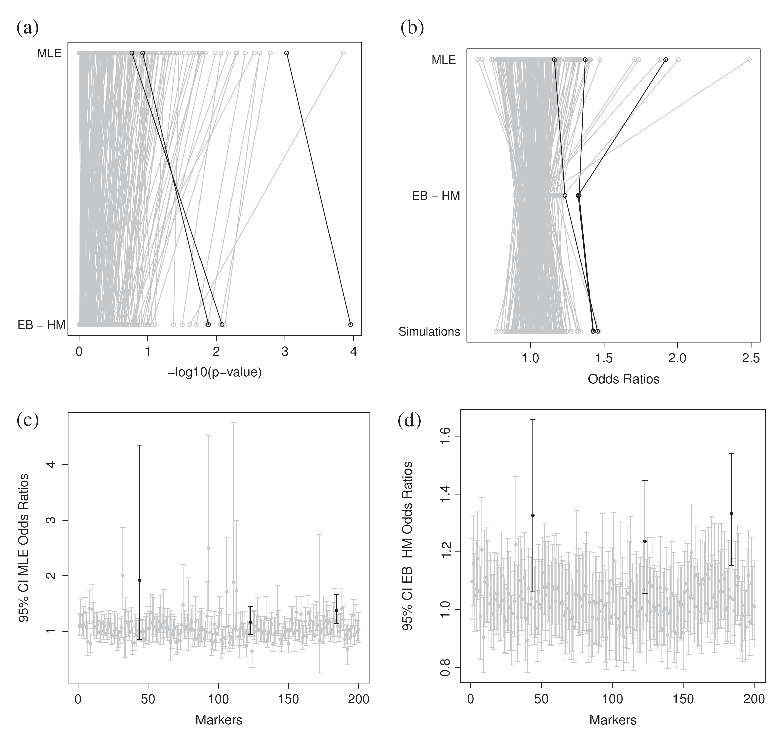
\includegraphics{fig1.eps}
\caption{Results of a simulation study with 200 markers,
for each of 500 cases and 500 controls. Markers 44, 123,
and 184 are 3 random markers chosen to have higher odds
ratios, and these are indicated in black, all other markers
are in gray. The MAF for each marker was randomly simulated
from Uniform(0.01, 0.5). The same $Z$ matrix was used in both
the simulation and analysis phase. (a) For both the MLEs
and the empirical Bayes estimators (EB-HM),
$-\log_{10} (\hbox{\textit{P}-value})$ are shown.
(b) The true odds ratios used in the simulation study
together with MLE and empirical Bayes estimators of the odds
ratios. (c) Confidence intervals for the logistic regression
MLEs of the odds ratios. (d) Approximate confidence intervals
for the empirical-Bayes estimated odds ratios.}
\label{Fig1}
\end{figure}

\begin{figure}[!p]
\centering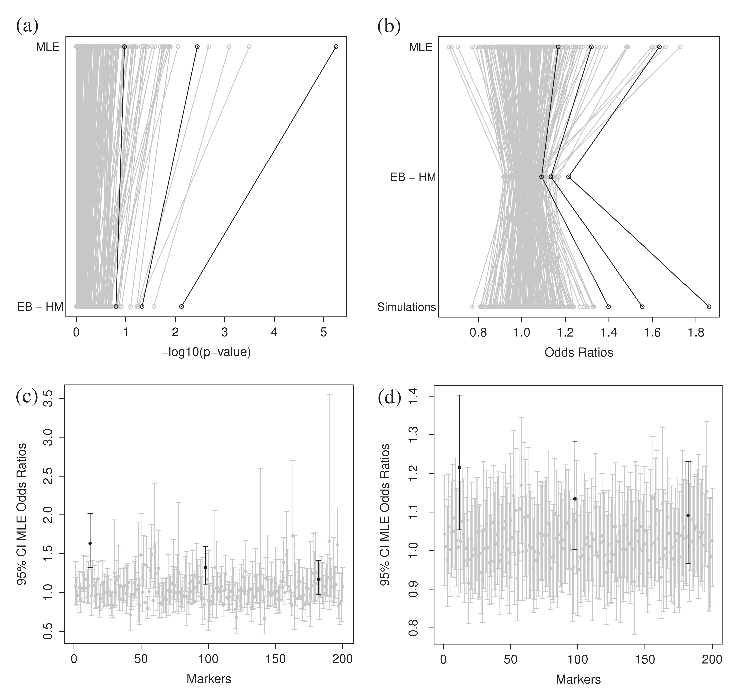
\includegraphics{fig2.eps}
\caption{Results of a simulation study with 200 markers,
for each of 500 cases and 500 controls. Markers 12, 98,
and 182 are 3 random markers chosen to have higher odds
ratios and these are indicated in black, all other
markers are in grey. The MAF for each marker was randomly
simulated from $\hbox{Uniform} (0.01, 0.5)$. An
alternative $Z$ matrix was used in the analysis phase
to that used in the simulation phase. (a) For both the
MLEs and the empirical Bayes estimators (EB-HM),
$-\log_{10} (\hbox{\textit{P}-value})$
are shown. (b) The true odds ratios used in the
simulation study together with MLEs and empirical Bayes
estimators of the odds ratios. (c) Confidence intervals
for the logistic regression MLEs of the odds ratios.
(d) Approximate confidence intervals for the empirical-Bayes
estimated odds ratios.}
\label{Fig2}
\end{figure}

\begin{figure}[!p]
\centering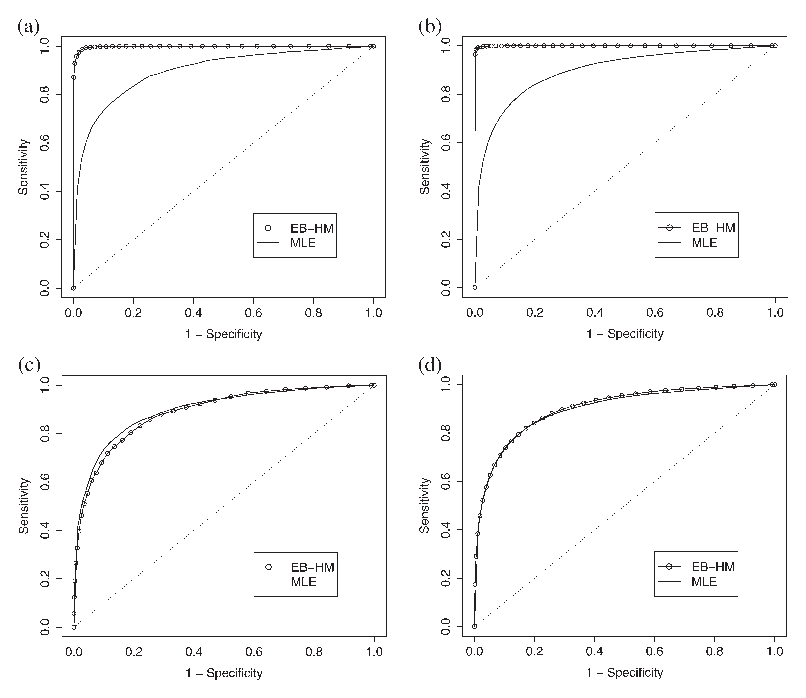
\includegraphics{fig3.eps}
\caption{(a) ROC curves for both MLE estimates and
EB-HM estimates based on 1000 random simulations of 500
cases and 500 controls, 200 markers with 2 causative
markers. Same $Z$ covariate matrix used in both generation
and analysis phases. (b) Same as plot (a) except 15
causative markers are simulated. (c) Same as (a) except
$Z$ is random positive noise
($\hbox{abs} [ \hbox{Normal} (0, 1) ]$) in the analysis
phase. (d) Same as plot (c) except 15 causative markers
are simulated.}
\label{Fig3}
\end{figure}

\begin{figure}[!p]
\centering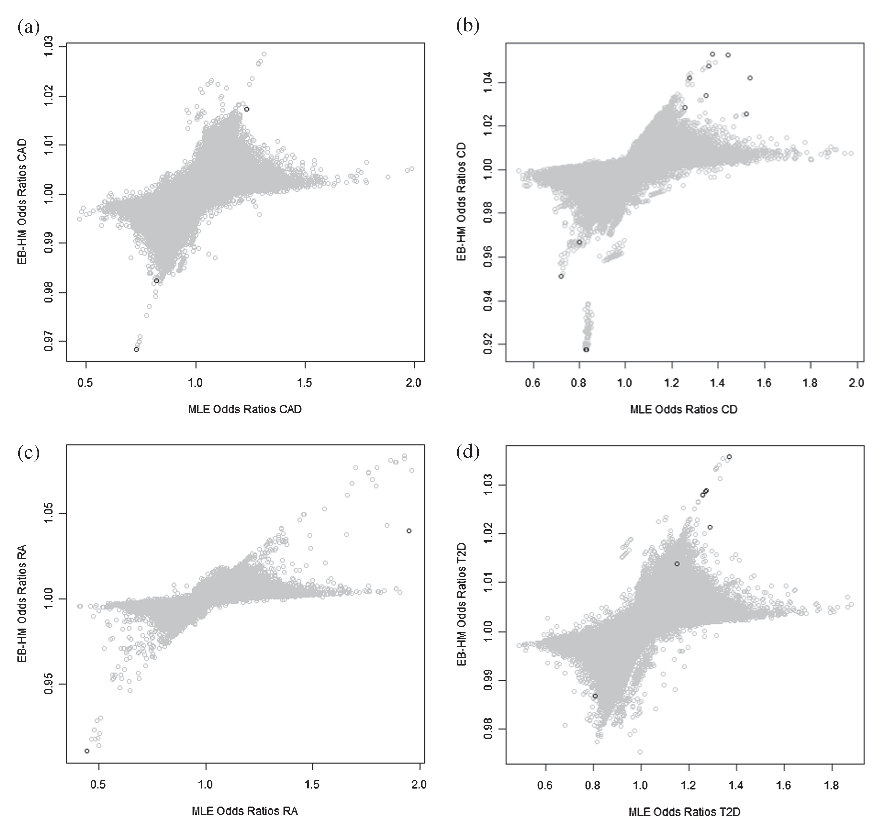
\includegraphics{fig4.eps}
\caption{MLE of the odds ratios (first-level logistic
regression model) and the empirical Bayes estimators
(EB-HM) of the odds ratios for the autosomal markers
(gray points) for (a) CAD, (b) CD, (c) RA, and (d) T2D.
Points in black are the markers detailed in Table
\protect\ref{Table1} for each of the disease data sets.}
\label{Fig4}
\end{figure}

\begin{table}[!p]
\tblcaption{A subset of the strongest associated
markers for each of the $4$
\protect\citet{rieger2004}
data sets (CAD, CD, RA, and T2D). MLE-OR(SE) refers
to the logistic regression maximum likelihood odds
ratio estimate and the standard error of the
$\log(\hbox{MLE OR})$ as calculated for the analysis
carried out here. MLE rank refers to the ranking
of the marker based on the MLE \textit{P}-value.
EB-HM-OR(SE) refers to the EB-HM odds ratio and the
standard error of the $\log(\hbox{EB-HM OR})$. The
EB-HM Rank refers to the rank of the marker based on
the EB-HM \textit{P}-value and the effect size (ES)
Rank refers to the ranking based on the EB-HM odds
ratios
\label{Table1}}
{\tabcolsep=4.25pt
\begin{tabular}{@{}cccccccccc@{}}
\tblhead{Dis & Chr & Marker & MLE-OR & MLE & MLE &
EB-HM-OR & EB-HM & EB-HM & ES \\
&&& (SE) & \textit{P}-value & rank & (SE) &
\textit{P}-value & rank & rank}
CAD & 2 & rs2943634 & 1.22(0.04) & $1.23 \times 10^{-5}$ &
32 & 1.02(0.01) & 0.19 & 28 & 37 \\
CAD & 6 & rs6922269 & 1.23(0.05) & $6.58 \times 10^{-6}$ &
22 & 1.02(0.01) & 0.2 & 37 & 44 \\
CAD & 9 & rs1333049 & 1.37(0.04) & $2.3 \times 10^{-14}$ &
1 & 1.03(0.01) & 0.016 & 1& 1 \\[3pt]
CD & 1 & rs11805303 & 1.37(0.04) & $8.1 \times 10^{-13}$ &
7 & 1.05(0.02) & 0.003 & 120 & 120 \\
CD & 2 & rs10210302 & 1.39(0.04) & $9.1 \times 10^{-14}$ &
2 & 1.05(0.02) & 0.004 & 123 & 123 \\
CD & 3 & rs9858542 & 1.26(0.05) & $8.16 \times 10^{-7}$ &
71 & 1.03(0.02) & 0.1 & 313 & 308 \\
CD & 5 & rs1000113 & 1.52(0.08) & $6.38 \times 10^{-8}$ &
48 & 1.03(0.02) & 0.169 & 701 & 512 \\
CD & 5 & rs17234657 & 1.54(0.06) & $3.34 \times 10^{-13}$ &
5 & 1.04(0.02) & 0.02 & 147 & 154 \\
CD & 10 & rs10761659 & 1.24(0.04) & $2.8 \times 10^{-7}$ &
61 & 1.03(0.02) & 0.05 & 221 & 211 \\
CD & 10 & rs10883365 & 1.28(0.04) & $1.53 \times 10^{-8}$ &
30 & 1.04(0.02) & 0.02 & 142 & 152 \\
CD & 16 & rs17221417 & 1.36(0.04) & $1.14 \times 10^{-11}$ &
16 & 1.05(0.02) & 0.008 & 128 & 128 \\
CD & 16 & rs2076756 & 1.44(0.05) & $8.35 \times 10^{-15}$ &
1 & 1.05(0.02) & 0.003 & 121 & 121 \\
CD & 17 & rs916793 & 1.2(0.05)\hphantom{0} & 0.0003 &
490 & 1.09(0.02) & $1.68 \times 10^{-6}$ & 2 & 2 \\
CD & 17 & rs17691328 & 1.21(0.05) & 0.0003 &
448 & 1.09(0.02) & $1.58 \times 10^{-6}$ & 1 & 1 \\
CD & 18 & rs2542151 & 1.35(0.05) & $5.1 \times 10^{-8}$ &
44 & 1.03(0.02) & 0.06 & 235 & 230 \\[3pt]
RA & 1 & rs6679677 & 1.95(0.06) & $2.86 \times 10^{-25}$ &
32 & 1.04(0.02) & 0.01 & 52 & 52 \\
RA & 6 & rs6457617 & 2.26(0.05) & $2.17 \times 10^{-72}$ &
1 & 1.1(0.02)\hphantom{0} & $1.38 \times 10^{-9}$ & 1 & 1 \\[3pt]
T2D & 3 & rs1801282 & 1.24(0.07) & 0.0013 &
761 & 1.01(0.01) & 0.38 & 2826 & 2228 \\
T2D & 6 & rs9465871 & 1.29(0.05) & $1.09 \times 10^{-6}$ &
19 & 1.02(0.01) & 0.15 & 42 & 42 \\
T2D & 10 & rs4506565 & 1.37(0.04) & $7.1 \times 10^{-13}$ &
1 & 1.04(0.01) & 0.02 & 1 & 1 \\
T2D & 11 & rs5215 & 1.15(0.04) & 0.00129 &
763 & 1.01(0.01) & 0.347 & 1779 & 1787 \\
T2D & 16 & rs7193144 & 1.27(0.04) & $1.56 \times 10^{-8}$ &
11 & 1.03(0.01) & 0.048 & 11 & 11 \\
T2D & 16 & rs8050136 & 1.27(0.04) & $2.16 \times 10^{-8}$ &
12 & 1.03(0.01) & 0.05 & 12 & 12 \\
T2D & 16 & rs9939609 & 1.26(0.04) & $5.6 \times 10^{-8}$ &
15 & 1.03(0.01) & 0.06 & 15 & 15
\lastline
\end{tabular}}
\end{table}

\end{document}

